\documentclass[12pt]{article}
\usepackage{amsmath}
\usepackage{latexsym}
\usepackage{amsfonts}
\usepackage{amssymb}
\usepackage{graphicx}
\usepackage{txfonts}
\usepackage{wasysym}
\usepackage{adjustbox}
\usepackage{ragged2e}
\usepackage{tabularx}
\usepackage{hhline}
\usepackage{float}
\usepackage{multirow}
\usepackage{makecell}
\usepackage{fancyhdr}
\usepackage[utf8]{inputenc}
\usepackage[T1]{fontenc}
\usepackage[a4paper,bindingoffset=0.2in,headsep=0.5cm,left=1in,right=1in,bottom=3cm,top=2cm,headheight=2cm]{geometry}
\usepackage{hyperref}
\usepackage{listings}

\everymath{\displaystyle}
\pagestyle{fancy}
\fancyhf{}
\rfoot{Page \thepage}
\begin{document}
\sloppy 

\begin{center}
\Large Telecom ParisTech \\
\Large TTool \\
\Large \url{ttool.telecom-paristech.fr}
\vspace{20 pt}\\
\underline{\Large Code generation from Avatar Design Diagrams in TTool}
\vspace{30 pt}
\end{center}

\begin{table}[H]
\large
\centering
\begin{adjustbox}{width=\textwidth}
\begin{tabular}{ |p{1.6cm}|p{6.0cm}|p{4.2cm}|p{4.2cm}| }
\hhline{----}
 & \textbf{Document Manager} & \textbf{Contributors}  & \textbf{Checked by}  \\ 
\hhline{----}
\textbf{Name}   & Ludovic APVRILLE & \multirow{2}{*}{Ludovic APVRILLE} &
\multirow{2}{*}{Ludovic APVRILLE} \\
\hhline{--~~}
\textbf{Contact} & ludovic.apvrille@telecom-paristech.fr &  &  \\ 
\hhline{--~~}
\textbf{Date} & \today &  &  \\ 
\hline
\end{tabular}
\end{adjustbox}
\end{table}

\newpage
\tableofcontents

% \newpage
% \listoffigures

\newpage
\section{Preface}

\subsection{Table of Versions}

\begin{table}[H]
\large
\centering
\begin{adjustbox}{width=\textwidth}
\begin{tabular}{ |p{1.5cm}|p{2.5cm}|p{9.0cm}|p{3.0cm}| }
\hhline{----}
\textbf{Version} & \textbf{Date} & \textbf{Description  $  \&  $  Rationale of
Modifications} & \textbf{Sections Modified} \\
\hhline{----}
1.0 & 13/06/2017 & First draft &  \\ 
\hline
\end{tabular}
\end{adjustbox}
\end{table}

\subsection{Table of References and Applicable Documents}

\begin{table}[H]
\large
\centering
\begin{adjustbox}{width=\textwidth}
\begin{tabular}{ |p{2.66in}|p{2.66in}|p{0.95in}|p{0.43in}| }
\hhline{----}
\textbf{Reference} & \textbf{Title  $  \&  $  Edition} & \textbf{Author or
Editor} & \textbf{Year}
\\
\hhline{----}
 &  &  &  \\ 
\hline
\end{tabular}
\end{adjustbox}
\end{table}

\subsection{Acronyms and glossary}

\begin{table}[H]
\large
\centering
\begin{adjustbox}{width=\textwidth}
\begin{tabular}{ |p{1.24in}|p{5.45in}| }
\hhline{--}
\textbf{Term} & \textbf{Description} \\ 
\hhline{--}
 &  \\ 
\hline
\end{tabular}
\end{adjustbox}
\end{table}

\subsection{Summary}

This document describes the code generation principle for AVATAR design diagrams implemented in TTool. It describes how to configure TTool for generating code, how to generate the code, how to compile it, how to execute it.
Finally, the document explains how to have the generated code to connect with an external graphical interface.

\section{Configuration}
\subsection{TTool configuration}
\label{sec:conf}
At first, if not already configured\footnote{TTool should be provided with the configuration already done}, you must open the configuration file of TTool. The default file is located in:
\begin{verbatim}
TTool/bin/config.xml
\end{verbatim}
Open your configuration file, and set the following lines accordingly with your TTool installation:
\begin{itemize}
\item Main directory in which the generated code and the avatar runtime library are located:
\begin{verbatim}
<AVATARExecutableCodeDirectory data="../executablecode/" />
\end{verbatim}
\item Host to connect to perform the code compilation and execution. Default value is "localhost".
\begin{verbatim}
<AVATARExecutableCodeHost data="localhost"/>
\end{verbatim}
\item Compilation command to compile the generated code:
\begin{verbatim}
<AVATARExecutableCodeCompileCommand data="make -C ../executablecode/" />
\end{verbatim}
\item Execution command. This will start the application generated from your model:
\begin{verbatim}
<AVATARExecutableCodeExecuteCommand data="../executablecode/run.x" />
\end{verbatim}
\end{itemize}

\subsection{External tools}
The previous configuration assumes that a \textbf{c compiler}, referenced by the provided Makefile (default = "gcc") is installed on your machine, as well as the \textbf{POSIX-1 librairies}. Also, a Mafile utility must be installed (e.g., "gnu make").

\section{A first example}
This very first example explains how to generate the code from an AVATAR design model, and how to introduce your own basic C directive in the code generation process.

\subsection{Getting the example}
Be sure to get the latest version of TTool including the remote loading of models (June 2017 and after). Do: File, Open from TTool repository, and select "HelloWorldCodeGeneration.xml".

\subsection{Understanding the model}
This models contains a design diagram composed of one MainBlock. This later regularly executes the "printHelloWorld" method (see Figure \ref{fig:printhelloworld}).


\begin{figure*}[htbp]
\centering
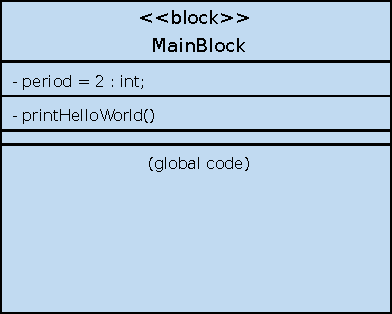
\includegraphics[scale=0.65]{figures/bdhelloworld.pdf}
\hspace{1cm}
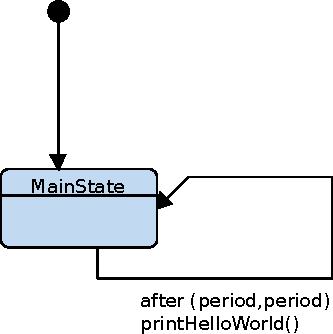
\includegraphics[Width]{figures/smdhelloworld.pdf}
\caption{Hello world model} \label{fig:printhelloworld}
\end{figure*}

You may then check the syntax of the diagram, and select the "interactive simulation icon". From the window that opens, make a step by step simulation, and observe the behaviour of the system. This behaviour is simulated, that is, there is no executable code that is generated to execute the system.

\begin{figure*}[htbp]
\centering
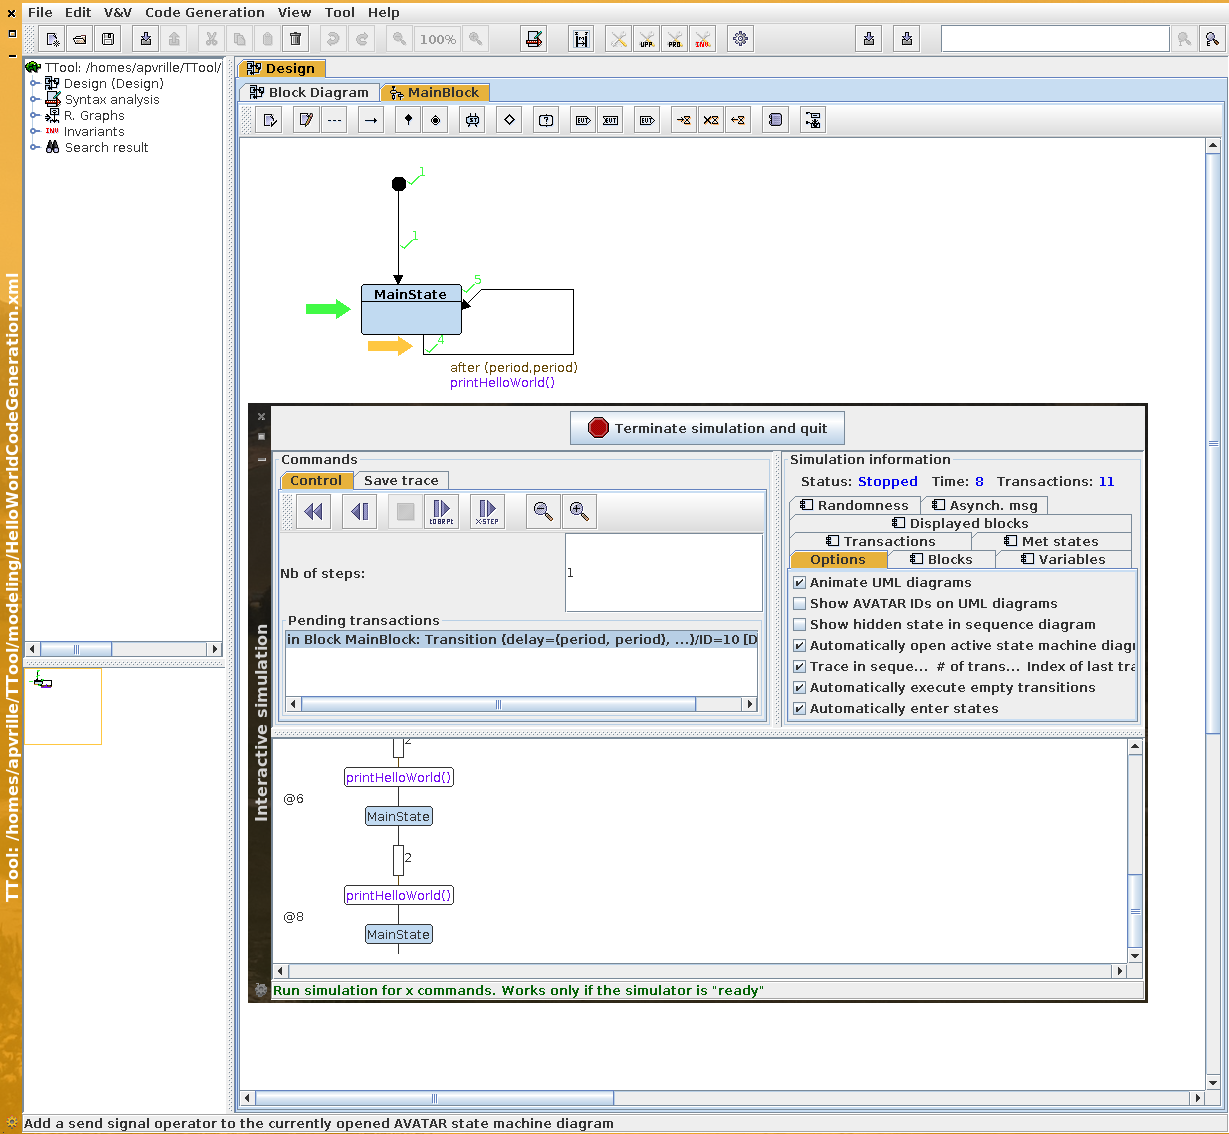
\includegraphics[width=1\textwidth]{figures/simulationhelloworld}
\caption{Functional simulation of the Hello world model} \label{fig:simuhelloworld}
\end{figure*}

\subsection{Generating executable code}
To generate executable code,








\end{document}
